\documentclass[conf]{new-aiaa}
%\documentclass[journal]{new-aiaa} for journal papers
\usepackage[utf8]{inputenc}

\usepackage{graphicx}
\usepackage{amsmath}
\usepackage[version=4]{mhchem}
\usepackage{siunitx}
\usepackage{longtable,tabularx}
\usepackage{footnote}
\usepackage{mhchem}
\usepackage{physics}
\usepackage{array,makecell,booktabs}
\newcolumntype{M}[1]{>{\centering\arraybackslash}m{#1}}
\usepackage[super]{nth}
\makesavenoteenv{tabular}
\setlength\LTleft{0pt}

\graphicspath{{figures/}}

\begin{document}

\section{Cost Model}

The TRANSCOST 8.2 model was implemented to evaluate the costs of different first stage reuse strategies \cite{transcost}. TRANSCOST is a top-down cost estimating model that utilizes historical data for similar projects to estimate the cost of launch vehicle elements. A series of cost estimation relationships (CERs) of the form $C = a M^x$ relate the mass $M$ of launch vehicle elements to their production costs using the empirically fitted parameters $a$ and $x$. Costs of all launch vehicle elements are then summed to determine the total launch vehicle production cost. 

The cost and performance models are linked through the launch vehicle element masses. For a given payload mass, the performance model can estimate the mass of launch vehicle elements for various first stage reuse strategies. These masses are then used with the cost model to estimate the production cost and cost per flight of those strategies. 

\subsection{Cost Model Description}

The TRANSCOST model considers three separate cost areas for launch vehicles: development, production, and operations costs \cite{transcost}. The cost per flight of a launch vehicle is the cost paid by the launch service provider for each flight, which includes production and operations costs only. The price per flight is the price paid by a customer to the launch service provider. This includes production and operations costs, as well as profit for the launch service provider and a potential development amortization charge. It should be noted, however, that typically a large part of development costs are funded by government contracts, such as for the Falcon 9 and Ariane 5 launch vehicles \cite{NASAspaceX, ESAAriane5}. In these cases, a development amortization charge is substantially reduced or not included as part of the price per flight.

It is interesting to look at the breakdown of costs in the cost per flight of a launch vehicle. Consider a two stage fully expendable launch vehicle utilizing kerosene and liquid oxygen propellants to carry a 10,000 kg payload to LEO. The cost per flight breakdown for such a launch vehicle can be seen in Figure \ref{fig:expendable_cost_breakdown}. 

\begin{figure}[hbt!]
    \centering
    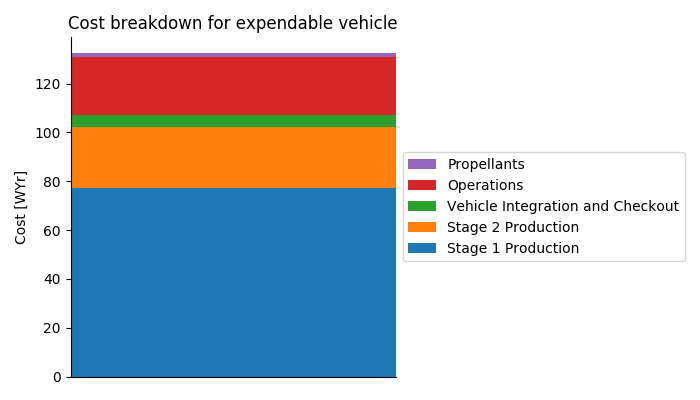
\includegraphics[width=0.7\textwidth]{../../lvreuse/analysis/combined/plots/expendable_cost_breakdown}
    \caption{\label{fig:expendable_cost_breakdown} Cost per flight breakdown for two stage fully expendable vehicle.}
\end{figure}

For this launch strategy -- and similarly for most fully expendable launch vehicle strategies -- the cost per flight is dominated by the first stage production costs. These large first stage production costs motivate strategies for first stage reusability, which would allow the first stage production cost to be amortized over a number of flights, therefore potentially reducing the total cost per flight. 

\subsection{Validation of Cost Model}

In order to validate the TRANSCOST model, the prices per flight for several current launch vehicles were evaluated with the model and compared to their actual advertised launch prices. As with the performance model, uncertainty in the cost model is accounted for using Monte Carlo methods. Credible range estimates for various cost parameters are used to establish parameter distributions. These distributions are then sampled to evaluate the cost model, generating a collection of cost model outputs that represent a range of credible cost estimates.

It should be noted that the TRANSCOST model as published only gives point estimates of launch vehicle costs, and provides no quantification for uncertainty in the model itself. The coefficients $a$ and $x$ in the element cost estimation relationships $C = a M^x$ are simply derived by curve fitting to historical reference data. In order to account for cost model uncertainty, we refit the reference data to the element CERs, extracting confidence bounds for each CER coefficient so that we can establish uncertainty distributions to sample. 

Four launch vehicles were used to evaluate the TRANSCOST model: Atlas V 401, Ariane 5G, Delta IV Medium (4,0), and Falcon 9 Block 3. The price per flight estimates for each were evaluated, including production costs, operations costs, and nominal profit, excluding any development amortization charges. The results, along with available price per flight data, are shown as a violin plot in Figure \ref{fig:vehicle_ppf_validation} \cite{ULARocketBuilder, FlightGlobalArianespace, GAO2017, SpaceXCapabilities}. 

\begin{figure}[hbt!]
    \centering
    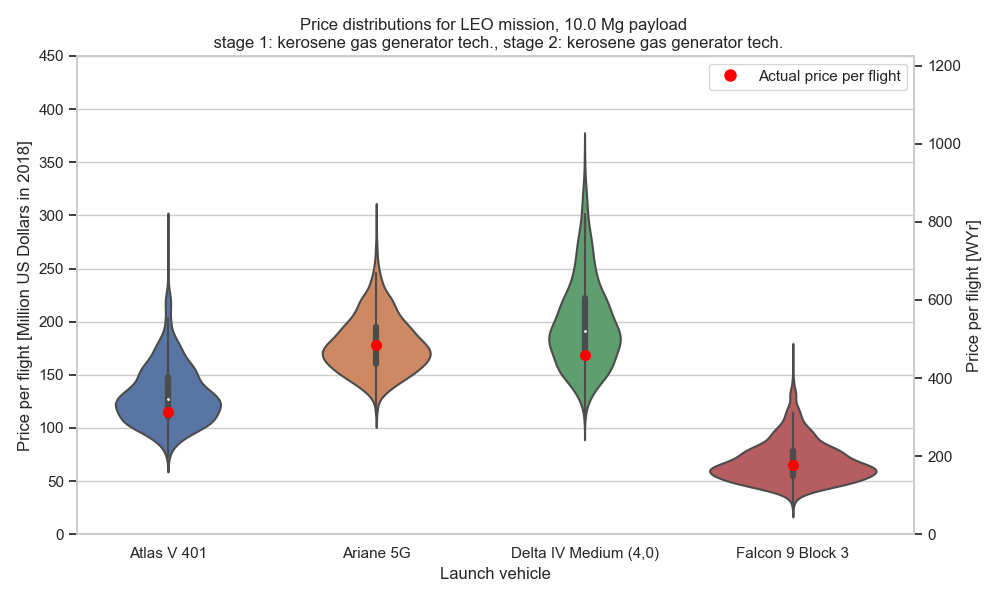
\includegraphics[width=\textwidth]{../../lvreuse/analysis/cost/plots/vehicle_ppf_validation}
    \caption{\label{fig:vehicle_ppf_validation} Distributions of price per flight estimates for several launch vehicles. Available actual price per flight information is included for comparison.}
\end{figure}

The price estimate distributions for these four vehicles are all reasonable, capturing the actual price per flight near the mode of the distribution. The distribution for Falcon 9 is predictably lower than the others, accounting for its high launch rate and SpaceX's lean manufacturing practices with minimal overhead costs. We see a slightly broader distribution of costs for the Delta IV launch vehicle, likely due to a few reasons. First, its use of the modern RS-68 engine on the first stage -- which has few similar reference projects for fitting of historical data -- requires a relatively broad confidence interval to characterize the CER coefficients. Second, the sensitivity of the launch vehicle costs to its learning factor is larger since the Delta IV is earlier in its program life than the other launch vehicles. These estimates lend credibility to the cost per flight estimates for the various first stage reuse strategies to be shown. 

\bibliography{first_stage_recovery}

\end{document}